%! TeX root = ../Parte1.tex

\section{Password}

\begin{myframe}{Data breach}
  Sebbene i server siano protetti, può capitare che un hacker/cracker vi acceda (ad esempio mediante una \emph{SQL injection}) e riesca a leggere i dati degli utenti.

  \pause\medskip
  I dati ottenuti vengono spesso venduti (dai cracker) ad aziende interessate oppure resi pubblici (dagli hacker) affinché i gestori del servizio riparino le falle e gli utenti cambino le proprie credenziali.
\end{myframe}

\begin{myframe}{Vendita dati}
    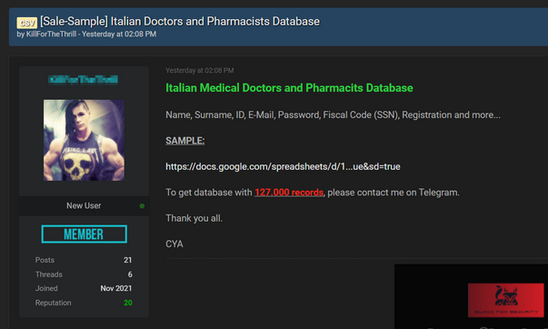
\includegraphics[width=.9\textwidth]{img/venditadati}
\end{myframe}
\begin{myframe}{Esempio data breach}
    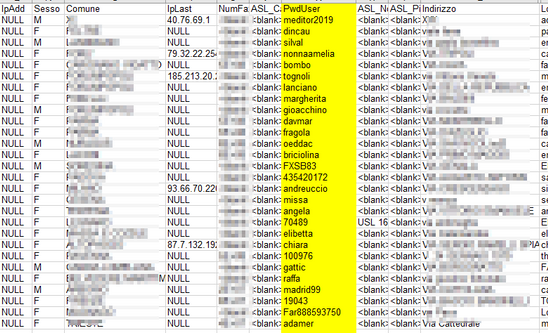
\includegraphics[width=.9\textwidth]{img/databreach}
\end{myframe}

\begin{myframe}{Firefox Monitor}
  Ci sono dei servizi gratuiti che ti informano se il tuo utente è stato violato, come \href{https://haveibeenpwned.com/}{Have I Been Pwned?} e \href{https://monitor.firefox.com/}{Firefox Monitor}.
  \begin{tikzpicture}
    \node at (0,0) {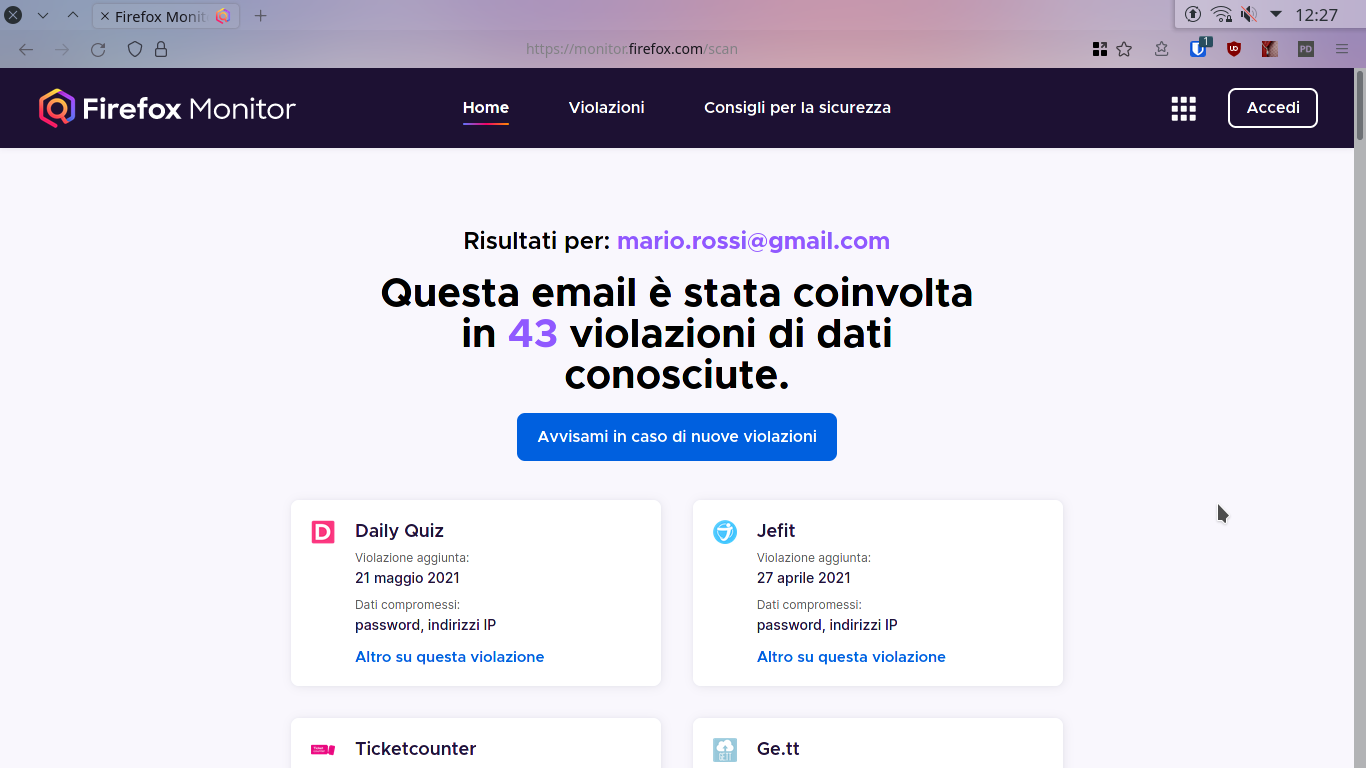
\includegraphics[width=\textwidth]{img/monitor}};
    \draw[gred, rounded corners] (-4,-1.7) node (A){} rectangle +(2,0.3);
    \draw[<-, gred] (A) +(0,0.15) -- +(-1.5,0.7) node[anchor=south] {Sito violato};
    \draw[gred, rounded corners] (-3.5,-2.65) node(B){} rectangle +(1.8,0.3);
    \draw[<-, gred] (B) +(0,0.15) -- +(-1.8,0.4) node[anchor=south] {Dati violati};
  \end{tikzpicture}
\end{myframe}

\begin{myframe}{Come vengono salvate le password sui server}
  Le password sui server non vengono salvate \textbf{in chiaro}, ma \textbf{criptate} (usando una funzione di hash).

  \pause\medskip
  Dalla password criptata non è possibile risalire alla password originale. Così se succede un \textbf{data breach} non è possibile ottenerle.

  \pause\medskip
  Per controllare se la password inserita al login è corretta si cripta la password inserita e si verifica che coincida con quella salvata già criptata.

  \texttt{cripta(password\_inserita) = password\_criptata ???}
\end{myframe}

\begin{myframe}{Le nostre password sono al sicuro?}
  \pause
  {\Huge\textbf{NO!}}
  \pause
  \only<+->{
    \medskip
    \begin{itemize}[<+(-1)->]
      \item Non tutti i siti criptano le password
      \item Alcune funzioni di criptazione sono obsolete (es. MD5): esistono delle tabelle che forniscono la funzione inversa
      \item Esistono dei tool (es. \href{https://www.openwall.com/john/}{John the Ripper}) che tentano di recuperare le password dalla loro versione criptata
    \end{itemize}
  }
\end{myframe}

\begin{myframe}{John the Ripper}
  Prova con tutte le password in un lista finché non trova quella giusta. È anche possibile generare password simili.

  \pause
  \vspace*{-12pt}
  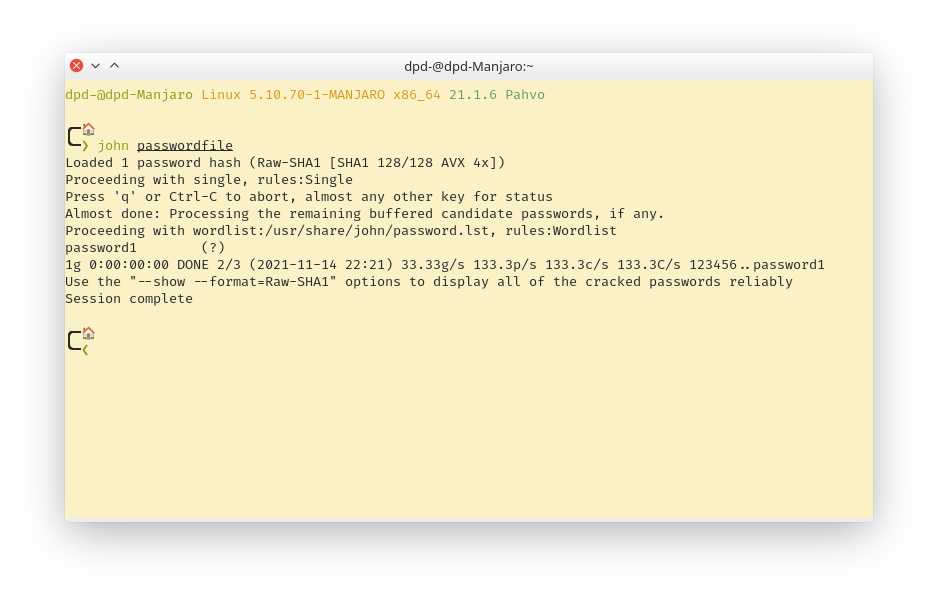
\includegraphics[width=.8\textwidth]{img/john}
  \vspace*{-19pt}

  \pause
  È quindi facile decriptare password che contengono parole comuni.
  % TODO Enigma
\end{myframe}

\begin{myframe}{Le password più usate}
  \pause
  \begin{itemize}[<+->]
    \item 1234, 123456, abc123
    \item password
    \item qwerty
    \item baseball, calcio
    \item letmein
    \item 111111
    \item uguale all'username
    \item data di nascita
  \end{itemize}

  \visible<+->{
    È quindi necessario creare delle \textbf{password robuste} che contengano lettere, numeri e simboli casuali.
  }

  \visible<+->{
    È anche importante non usare la stessa password per più di un servizio.
  }
\end{myframe}

\begin{myframe}{Come ricordarsi le password}
  Come fare a ricordarsi tante password così difficili?
  \pause
  \begin{itemize}[<+->]
    \item \stafter<.>{Le scrivo su un foglietto}
    \item \stafter<.>{Le scrivo su un file}
    \item \stafter<.>{Le salvo sul cloud}
    \item \stafter<.>{Le dico ad un amico}
    \item Uso un password manager: basta ricordarsi una password per saperle tutte
  \end{itemize}
\end{myframe}

\begin{myframe}{Bitwarden}
  Uno dei tanti password manager disponibili.

  \medskip\pause
  Gratuito ed open source.

  \medskip\pause
  \begin{itemize}
    \item Estensione per Browser
    \item App per telefono
    \item Programma per computer
  \end{itemize}
\end{myframe}

\begin{myframe}{Login con password manager}
  I password manager solitamente riconoscono i campi di login e le compilano automaticamente.

  \medskip\pause
  In caso contrario si può selezionare l'icona dell'estensione e cliccare sull'account giusto per la compilazione automatica.

  \begin{tikzpicture}
    \node at (0,0) {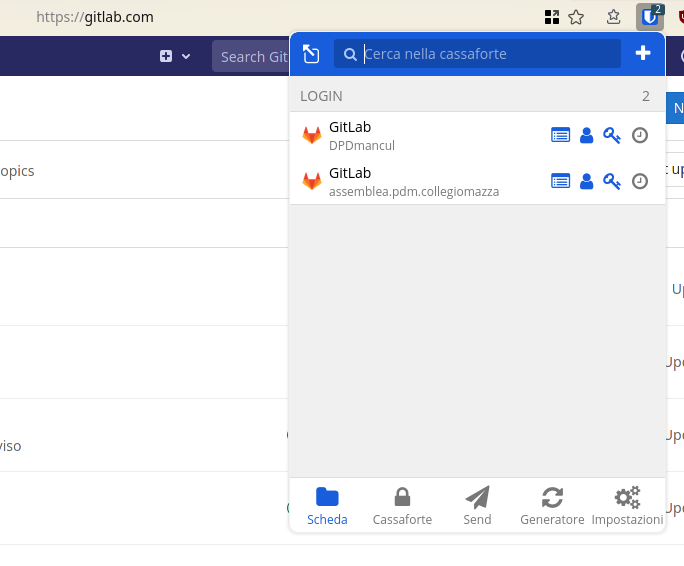
\includegraphics[width=.45\textwidth]{img/login}};
    \draw[<-, gred] (0,0.8) -- +(-2,-1) node[anchor=north] {Compilazione automatica};
    \draw[<-, gred] (1.9,0.8) -- +(-1,-0.5) node[anchor=north] {Mostra dati};
    \draw[<-, gred] (2.25,0.8) -- +(0,-1) node[anchor=north] {Copia username};
    \draw[<-, gred] (2.6,0.8) -- +(1,-0.5) node[anchor=north] {~~~Copia password};
  \end{tikzpicture}
\end{myframe}

\begin{myframe}{Login con password manager}
  Si integra anche con la compilazione automatica delle app
  \begin{figure}
    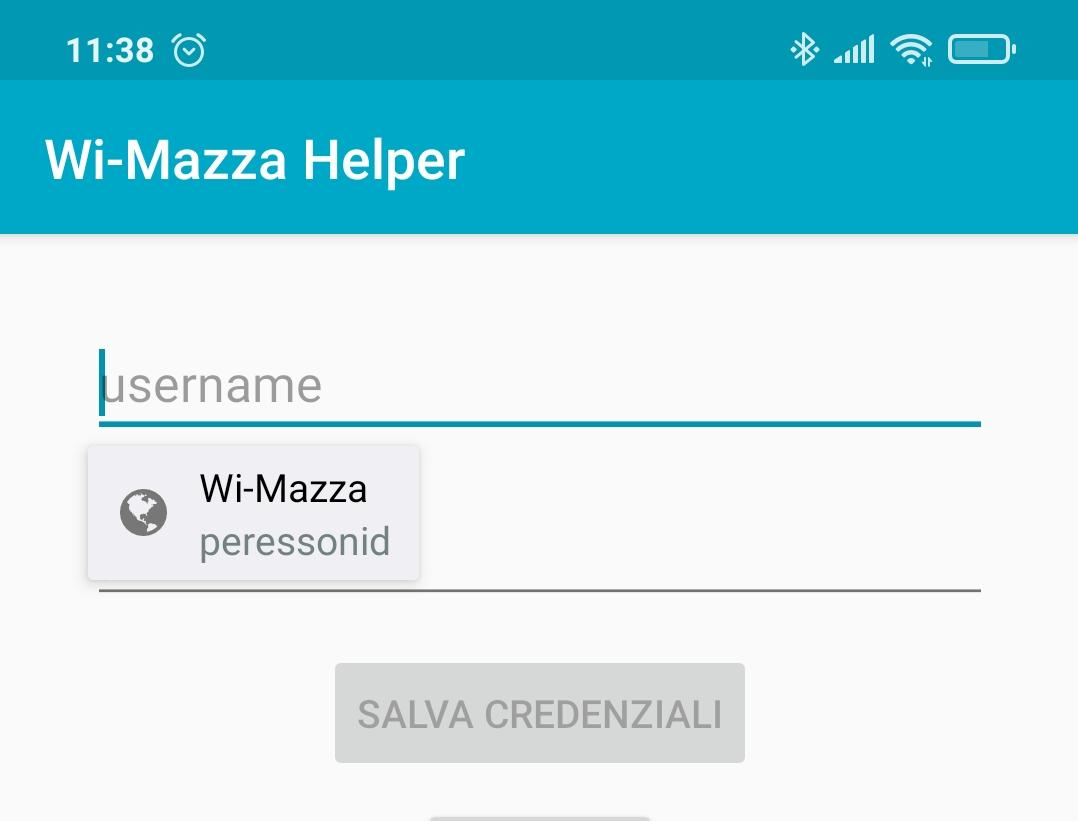
\includegraphics[width=.5\textwidth]{img/loginapp}
  \end{figure}
\end{myframe}

\begin{myframe}{Creare password sicure}
  \begin{figure}
    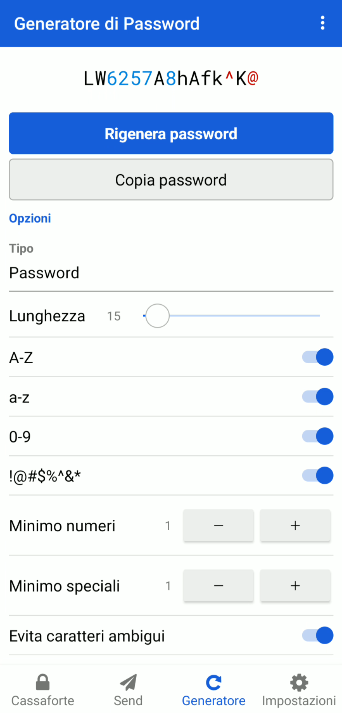
\includegraphics[height=.8\paperheight]{img/generatepass}
  \end{figure}
\end{myframe}

\begin{myframe}{Salvare le password}
  Quando ci si registra in un sito il password manager dovrebbe chiedere se vuoi salvare le credenziali:

  \begin{figure}
    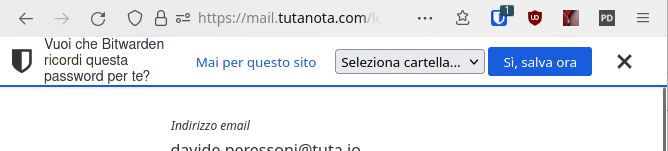
\includegraphics[width=\textwidth]{img/savepass}
  \end{figure}

  \medskip\pause
  In caso contrario è possibile salvarle manualmente.
\end{myframe}

\begin{myframe}{Altri vantaggi dei password manager}
  \begin{itemize}
    \item Difende da \textbf{keylogger}, non dovendo digitare la password;
    \item Difende da siti di \textbf{phishing}: la compilazione automatica funziona solo sul sito originale.
  \end{itemize}
\end{myframe}

\begin{myframe}{Passphrases}
  Quando non si può usare un password manager è meglio usare  le \textbf{passphrases}\\al posto delle password: sono più facili da ricordare e altrettanto sicure.

  \pause\bigskip
  gamma-pastel-head-astound-bottling-detached

  \pause\bigskip
  {\raggedright\textbf{Importante}\\}
  \begin{itemize}
    \item Le parole devono essere casuali (i password manager possono generarle)
    \item Devono esserci almeno 6 parole
    \item meglio cambiare una lettera a caso con un numero e una con un simbolo
  \end{itemize}
\end{myframe}

\begin{myframe}{Autenticazione a 2 fattori}
  Molti siti permettono di aggiungere un secondo step per il login, oltre alla password.
  \begin{itemize}
    \item OTP (one time password) via SMS;
    \item Token generato con apposita chiavetta;
    \item \dots
  \end{itemize}
\end{myframe}

\begin{myframe}{Controllo delle sessioni}
  È buona tenere d'occhio le sessioni attive per i nostri account per accertarsi che nessuno sia entrato al posto nostro.

  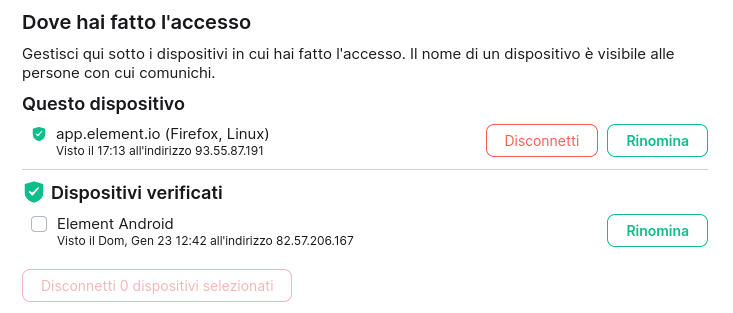
\includegraphics[width=.7\textwidth]{img/sessioni}

  \medskip\pause
  In caso di intrusione disabilitare subito la sessione e cambiare radicalmente password!
\end{myframe}
